\documentclass[review]{elsarticle} %review=doublespace preprint=single 5p=2 column
%%% Begin My package additions %%%%%%%%%%%%%%%%%%%
\usepackage[hyphens]{url}

  \journal{An awesome journal} % Sets Journal name


\usepackage{lineno} % add
\providecommand{\tightlist}{%
  \setlength{\itemsep}{0pt}\setlength{\parskip}{0pt}}

\usepackage{graphicx}
\usepackage{booktabs} % book-quality tables
%%%%%%%%%%%%%%%% end my additions to header

\usepackage[T1]{fontenc}
\usepackage{lmodern}
\usepackage{amssymb,amsmath}
\usepackage{ifxetex,ifluatex}
\usepackage{fixltx2e} % provides \textsubscript
% use upquote if available, for straight quotes in verbatim environments
\IfFileExists{upquote.sty}{\usepackage{upquote}}{}
\ifnum 0\ifxetex 1\fi\ifluatex 1\fi=0 % if pdftex
  \usepackage[utf8]{inputenc}
\else % if luatex or xelatex
  \usepackage{fontspec}
  \ifxetex
    \usepackage{xltxtra,xunicode}
  \fi
  \defaultfontfeatures{Mapping=tex-text,Scale=MatchLowercase}
  \newcommand{\euro}{€}
\fi
% use microtype if available
\IfFileExists{microtype.sty}{\usepackage{microtype}}{}
\bibliographystyle{elsarticle-harv}
\usepackage{graphicx}
\ifxetex
  \usepackage[setpagesize=false, % page size defined by xetex
              unicode=false, % unicode breaks when used with xetex
              xetex]{hyperref}
\else
  \usepackage[unicode=true]{hyperref}
\fi
\hypersetup{breaklinks=true,
            bookmarks=true,
            pdfauthor={},
            pdftitle={Short Paper},
            colorlinks=false,
            urlcolor=blue,
            linkcolor=magenta,
            pdfborder={0 0 0}}
\urlstyle{same}  % don't use monospace font for urls

\setcounter{secnumdepth}{0}
% Pandoc toggle for numbering sections (defaults to be off)
\setcounter{secnumdepth}{0}


% Pandoc header

\usepackage[nomarkers]{endfloat}
\linenumbers
\usepackage{setspace}
\doublespacing

\begin{document}
\begin{frontmatter}

  \title{Short Paper}
    \author[Some Institute of Technology]{Alice Anonymous\corref{1}}
   \ead{alice@example.com} 
    \author[Another University]{Bob Security}
   \ead{bob@example.com} 
    \author[Another University]{Cat Memes\corref{2}}
   \ead{cat@example.com} 
    \author[Some Institute of Technology]{Derek Zoolander\corref{2}}
   \ead{derek@example.com} 
      \address[Some Institute of Technology]{Department, Street, City, State, Zip}
    \address[Another University]{Department, Street, City, State, Zip}
      \cortext[1]{Corresponding Author}
    \cortext[2]{Equal contribution}
  
  \begin{abstract}
  \hypertarget{abstract}{%
  \section{Abstract}\label{abstract}}
  
  Noise, as the term itself suggests, is most often seen a nuisance to
  ecological insight, a inconvenient reality that must be acknowledged, a
  haystack that must be stripped away to reveal the processes of interest
  underneath. Yet despite this well-earned reputation, noise is often
  interesting in its own right: noise can induce novel phenomena that
  could not be understood from some underlying determinstic model alone.
  Nor is all noise the same, and close examination of differences in
  frequency, color or magnitude can reveal insights that would otherwise
  be inaccessible. Yet with each aspect of stochasticity leading to some
  new or unexpected behavior, the time is right to move beyond the
  familiar refrain of ``everything is important'' (Harrison et al., 2019).
  Stochastic phenomena can suggest new ways of inferring process from
  pattern, and thus spark more dialog between theory and empirical
  perspectives that best advances the field as a whole. I highlight a few
  compelling examples, while observing that the study of stochastic
  phenomena are only beginning to make this translation into empirical
  inference. There are rich opportunities at this interface in the years
  ahead.
  
  \newpage
  \end{abstract}
  
 \end{frontmatter}

\hypertarget{introduction}{%
\section{Introduction}\label{introduction}}

This is my awesome introduction that clearly defines the context and the
gaps I am going to address with this beautiful paper. I will also states
the hypotheses that I will test. It is going to be great, yeah yeah.

This introduction is going good, yes indeed, it will. And as it has been
proven before (Harrison et al., 2019; Ho and Budescu, 2019), this has
not been proven before. Evennnn better!

\newpage

\hypertarget{methods}{%
\section{Methods}\label{methods}}

So I used a very cool method (Ho and Budescu, 2019). Yeah yeah, but see
also (Harrison et al., 2019). Oh and there is also (Salih et al., 2000),
or (Baird et al., 2018).

Here is the model I used (it is an awesome model):

\begin{align}
\frac{\mathrm{d} n}{\mathrm{d} t} = \underbrace{c n \left(1 - \frac{n}{N}\right)}_{\textrm{birth}} - \underbrace{e n}_{\textrm{death}}, \label{levins}
\end{align}

\newpage

\hypertarget{results}{%
\section{Results}\label{results}}

We can see that the variables increase and plato to a maximum value
(Figure \ref{fig:figure1}). But my favorite figure is Figure
\ref{fig:myfigure}.

\hypertarget{discussion}{%
\section{Discussion}\label{discussion}}

\hypertarget{acknowledgements}{%
\section{Acknowledgements}\label{acknowledgements}}

The author acknowledges feedback and advice from the editor, Tim Coulson
and two anonymous reviewers. This work was supported in part by USDA
National Institute of Food and Agriculture, Hatch project
CA-B-INS-0162-H.

\hypertarget{references}{%
\section{References}\label{references}}

\newpage

\textbackslash{}begin\{landscape\}

\begin{figure}

{\centering 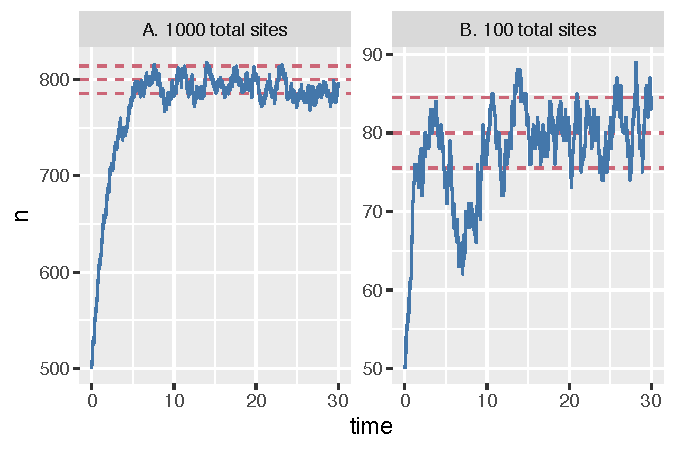
\includegraphics[angle=0]{My_Ecology_Letters_article_files/figure-latex/figure1, figure1-1} 

}

\caption{\label{fig:figure1}Population dynamics from a Gillespie simulation of the Levins model with large (N=1000, panel A) and small (N=100, panel B) number of sites (blue) show relatively weaker effects of demographic noise in the bigger system. Models are otherwise identical, with e = 0.2 and c = 1 (code in appendix A). Theoretical predictions for mean and plus/minus one standard deviation shown in horizontal re dashed lines.}\label{fig:figure1, figure1}
\end{figure}

\begin{figure}
\centering
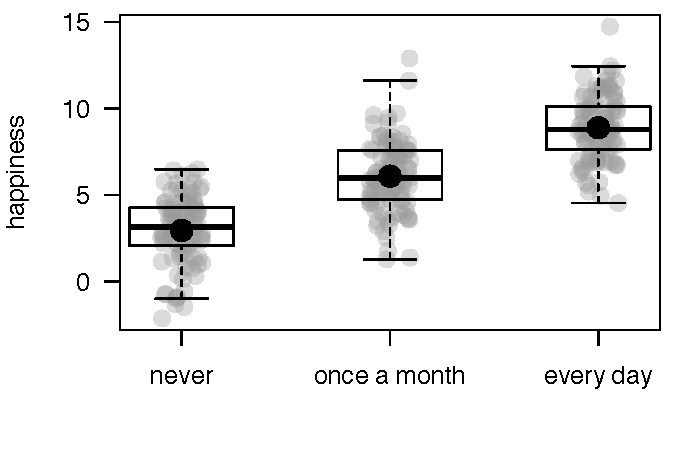
\includegraphics{My_Ecology_Letters_article_files/figure-latex/myfigure-1.pdf}
\caption{\label{fig:myfigure}The is my figure. It is awesome. Plus it
does not use ggplot, which is even better. It shows the level of
happiness relatively to the amount of cheese people eat.}
\end{figure}

\textbackslash{}end\{landscape\}

\hypertarget{refs}{}
\leavevmode\hypertarget{ref-baird_effects_2018}{}%
Baird, A., Álvarez-Noriega, M., Cumbo, V., Connolly, S., Dornelas, M.,
Madin, J., 2018. Effects of tropical storms on the demography of reef
corals. Mar. Ecol. Prog. Ser. 606, 29--38.
doi:\href{https://doi.org/10.3354/meps12760}{10.3354/meps12760}

\leavevmode\hypertarget{ref-harrison_back_2019}{}%
Harrison, H.B., Álvarez-Noriega, M., Baird, A.H., Heron, S.F.,
MacDonald, C., Hughes, T.P., 2019. Back-to-back coral bleaching events
on isolated atolls in the Coral Sea. Coral Reefs 38, 713--719.
doi:\href{https://doi.org/10.1007/s00338-018-01749-6}{10.1007/s00338-018-01749-6}

\leavevmode\hypertarget{ref-ho_climate_2019}{}%
Ho, E.H., Budescu, D.V., 2019. Climate uncertainty communication. Nat.
Clim. Chang. 9, 802--803.
doi:\href{https://doi.org/10.1038/s41558-019-0606-6}{10.1038/s41558-019-0606-6}

\leavevmode\hypertarget{ref-salih_fluorescent_2000}{}%
Salih, A., Larkum, A., Cox, G., Kühl, M., Hoegh-Guldberg, O., 2000.
Fluorescent pigments in corals are photoprotective. Nature 408,
850--853. doi:\href{https://doi.org/10.1038/35048564}{10.1038/35048564}


\end{document}


